\documentclass[../../main.tex]{subfiles}
    
    \lstset{basicstyle=\small,
      showstringspaces=false,
      commentstyle=\color{black},
      keywordstyle=\color{blue}
    }
    
    \graphicspath{{images/Fahrdaten/}{../../images/Fahrdaten/}}

    \begin{document}
    \subsection{Fahrdaten: Beschleunigung} \label{fahr_beschleunigung}
    In der Anforderungsliste ist es gefordert, dass die Systemsteuerung die Aktuellen Fahrdaten auswerten kann. Dazu ist es nötig, dass die Daten von Sensoren aufgenommen werden. Diese Daten sollen dann an die Systemsteuerung geschickt werden. In diesem Kapitel werden die Möglichkeiten zur Erfassung der Beschleunigung gezeigt. Mit der Beschleunigung kann man auch auf die Fliehkräfte schliessen. Die Daten der Fliehkräfte können von der Steuerung für eine optimale Kurvenfahrt benutzt werden.

    \textbf{Übersicht Konzepte}\\
    Es werden der verschiedene Ansätze mit verschiedenen Sensoren betrachtet. Zu jeder Möglichkeit werden Vor- und Nachteile aufgelistet und Risiken analysiert.
    Beschleunigungssensoren sind in diversen Varianten verfügbar. Vom Funktionsprinzip unterscheiden sie sich aber kaum. Deshalb werden hier nur folgende Möglichkeiten betrachtet. Der genaue Sensor wird dann durch die Wahl des Controllerboards und dessen Kommunikationsmöglichkeiten bestimmt.
    \begin{itemize}
        \item Onboard Sensorik
        \item Third Party Sensorik
    \end{itemize}

    \subsubsection{Onboard Sensorik}
    Viele Entwicklungsboards sind bereits mit einigen Sensoren bestückt. Vielfach ist auch ein Beschleunigungssensor dabei.

    \begin{flushleft}
        \begin{table}[H]
        \begin{tabular}{ | l | p{11cm} |}
        \hline
        \textbf{Problemstellung} & Fahrdaten: Beschleunigung \\ \hline
        \textbf{Disziplin} & Elektrotechnik \\ \hline
        \textbf{Lösungskonzept} & Onboard Sensorik\\ \hline
        \textbf{Komponente} & \begin{itemize}
            \item NXP Freedom Board FRDM-K22F
            \item FXOS8700CQ – accelerometer and magnetometer (auf Board vorhanden)
            \end{itemize}\\ \hline
        \textbf{Bewertung} &  \begin{itemize}
                                \item[+] keine weitere Hardware für Sensor nötig
                                \item[+] kleineres Risiko für Störungen durch kurze Leitungen
                                \item[-] Einschränkung in der Wahl der Steuerung und des Sensors
                                \item[-] gedämpfte Lagerung des Sensors nicht möglich
                              \end{itemize} \\ \hline
        \end{tabular}
        \caption{Konzeptbeurteilung: Beschleunigung Onboard Sensorik}
        \label{tab:fahr_Onboard_Sensorik}
    \end{table}
    \end{flushleft}

    \subsubsection{Third Party Sensorik}
    Für diese Möglichkeit wird der Sensor als einzelkomponente eingekauft und im Zug verbaut. Dies kann auf einem separaten PCB oder als einzelnes IC sein. 

    \begin{flushleft}
        \begin{table}[H]
        \begin{tabular}{ | l | p{11cm} |}
        \hline
        \textbf{Problemstellung} & Fahrdaten: Beschleunigung \\ \hline
        \textbf{Disziplin} & Elektrotechnik \\ \hline
        \textbf{Lösungskonzept} & Third Party Sensorik\\ \hline
        \textbf{Komponente} & \begin{itemize}
            \item GY LSM303 Breakout
            \item evt. zusätzliche Beschaltung
            \end{itemize}\\ \hline
        \textbf{Bewertung} &  \begin{itemize}
                                \item[+] Freie Wahl von Sensor und Controllerboards
                                \item[+] optimalere Platzausnutzung möglich 
                                \item[-] grösseres Risiko für Störungen durch längere Leitungen
                                \item[-] evt. zusätzliche Beschaltung vom Sensor nötig 
                              \end{itemize} \\ \hline
        \end{tabular}
        \caption{Konzeptbeurteilung: Beschleunigung Third Party Sensorik}
        \label{tab:fahr_Third_Party_Sensorik}
    \end{table}
    \end{flushleft}

    \subsubsection{Entscheid}
    Mithilfe der Nutzwertanalyse in Abbildung \ref{fig:fahr_nutzwertanalyse_beschleunigung} konnte ein Entscheid getroffen werden.\\
    Da auf den Ausgewählten Controllerboards, Raspberry Pi und Tiny K22, keine Onboard Sensorik zur Verfügung setehen bleibt nur die Wahlt von Third Party Sensorik. Deshalb ist Machbarkeit der Onboard Sensorik mit Null Punkten bewertet.\\
    Die Sensorik kann dann mit den Controllerboards verbunden werden und mit diesen Kommunizieren.\\
    Das Risiko für Störungen kann minimiert werden indem die Sensoren durch möglichst kurze Leitungen mit den Controllerboards verbunden werden. Mit dieser Wahl ist es auch möglich eine gedämpfte Lagerung der Sensorik zu realisieren. Damit können Messfehler z.B. von Unebenheiten der Strecke minimiert werden.  
        
    \begin{figure}[H]
        \centering
        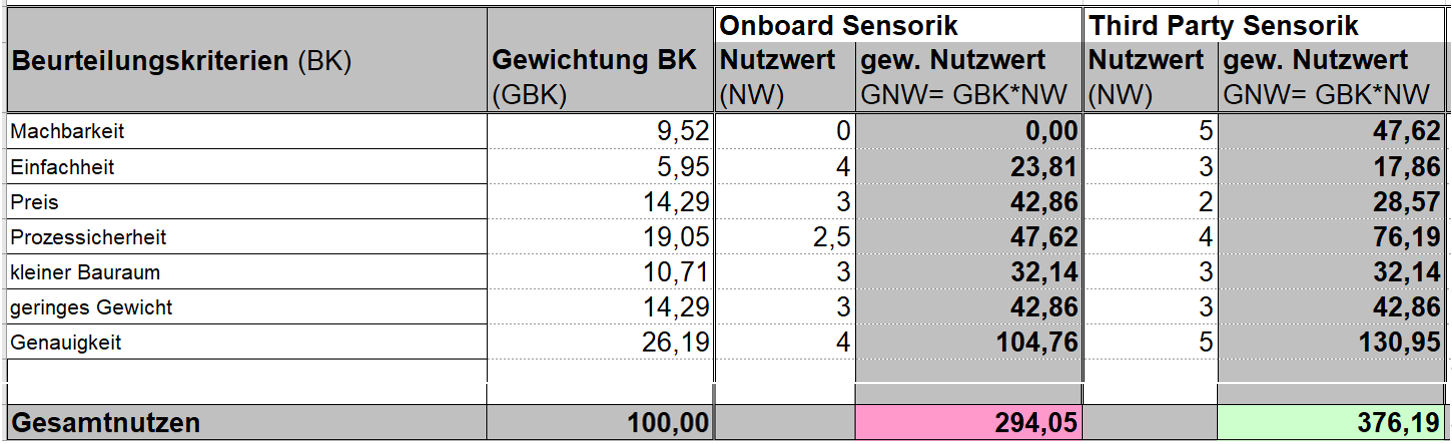
\includegraphics[width=1.0\textwidth]{Nutzweranalyse_Fahrdaten_Beschleunigung.png}
        \caption {Nutzwertanalyse Fahrdaten Beschleunigung}
        \label{fig:fahr_nutzwertanalyse_beschleunigung}
    \end{figure}

    \subsection{Fahrdaten: Geschwindigkeit} \label{fahr_geschwindigkeit}
    In diesem Kapitel werden die Möglichkeiten zur Erfassung der Geschwindigkeit gezeigt. Diese kann durch Sensoren ermittelt werden oder mithilfe der Beschleunigung errechnet werden. (siehe \ref{fahr_beschleunigung})

    \textbf{Übersicht Konzepte}\\
    Es werden der verschiedene Ansätze mit verschiedenen Sensoren betrachtet. Zu jeder Möglichkeit werden Vor- und Nachteile aufgelistet und Risiken analysiert.
    Es werden Möglichkeit betrachtet die Geschwindigkeit mit Sensoren zu ermitteln und solche die Geschwindigkeit rechnerisch aus der Beschleunigung zu bestimmen.
    \begin{itemize}
        \item Auswertung über Gleise
        \item Encoder
        \item Verknüpfung Encoder und Beschleunigungssensor
    \end{itemize}

    \subsubsection{Auswertung über Gleise}
    Unter den Gleisen, senkrecht zur Fahrtrichtung, befinden sich Verbindungsstücke aus Kunststoff. Diese sind ca. 5mm hoch und 10mm breit und sind durchschnittlich mit einem Abstand von ca. 15 mm montiert. Mit einem Sensor können diese erfasst werden und durch die verstrichene Zeit zwischen zwei Verbindungsstücken kann die Geschwindigkeit berechnet werden.

    \begin{flushleft}
        \begin{table}[H]
        \begin{tabular}{ | l | p{11cm} |}
        \hline
        \textbf{Problemstellung} & Fahrdaten: Geschwindigkeit \\ \hline
        \textbf{Disziplin} & Elektrotechnik \\ \hline
        \textbf{Lösungskonzept} & Auswertung über Gleise\\ \hline
        \textbf{Komponente} & \begin{itemize}
            \item Distanzsensor
            \item Timer im Controller für Zeitmessung
            \end{itemize}\\ \hline
        \textbf{Bewertung} &  \begin{itemize}
                                \item[-] Sensor muss sehr kleine Distanzunterschiede erkennen können
                                \item[-] Risiko für Messfehler durch unterschiedlichen Abstand zwischen den Verbindungsstücken
                              \end{itemize} \\ \hline
        \end{tabular}
        \caption{Konzeptbeurteilung: Geschwindigkeit Auswertung über Gleise}
        \label{tab:fahr_Auswertung_Gleise}
    \end{table}
    \end{flushleft}

    \subsubsection{Encoder}
    Mit einem Encoder misst man die Umdrehungszahl des Motor oder der Räder. Dabei wird in regelmässigen Abständen ein Signal an den Conroller geschickt. Diese Signale werden immer bei den Selben Positionen in der Umdrehung des Motors oder der Räder erzeugt. Mit einer Zeitmessung zwischen diesen Signalen kann die Geschwindigkeit berechnet werden.

    \begin{flushleft}
        \begin{table}[H]
        \begin{tabular}{ | l | p{11cm} |}
        \hline
        \textbf{Problemstellung} & Fahrdaten: Geschwindigkeit \\ \hline
        \textbf{Disziplin} & Elektrotechnik \\ \hline
        \textbf{Lösungskonzept} & Encoder\\ \hline
        \textbf{Komponente} & \begin{itemize}
            \item Encoder am Motor oder Rad
            \item Timer im Controller für Zeitmessung
            \end{itemize}\\ \hline
        \textbf{Bewertung} &  \begin{itemize}
                                \item[+] Exakte Messung, da die Messpunkte regelmässige verteilt sind
                                \item[-] Risiko für Fehlmessung bei Schlupf
                              \end{itemize} \\ \hline
        \end{tabular}
        \caption{Konzeptbeurteilung: Geschwindigkeit Encoder}
        \label{tab:fahr_Encoder}
    \end{table}
    \end{flushleft}

    \subsubsection{Verknüpfung Encoder und Beschleunigungssensor}
    Zusätzlich zum Encoder kann die Geschwindigkeit über die Integration Beschleunigung bestimmt werden. Diesen Wert kann dann der Kontrolle der Daten des Encoders dienen.\\
    Unter der Annahme, dass zu beginn der Messung zum Zeitpunkt $t = 0$ die Geschwindigkeit $0$ ist $(v_0 = 0)$ kann die Geschwindigkeit zum Zeitpunkt $t$ bestimmt werden mit $$v(t) = \int_{0}^{t} a(x) dx$$.\\
    Da aber auf einem Digitalen System die Daten nur zu diskreten Zeitpunkten ausgewertet werden können ergibt sich dann eine Summen der Beschleunigungen zum Zeitpunkt $k$ $$v[k] = \sum_{i=0}^{k}a[i] \Delta t$$ 

    \begin{flushleft}
        \begin{table}[H]
        \begin{tabular}{ | l | p{11cm} |}
        \hline
        \textbf{Problemstellung} & Fahrdaten: Geschwindigkeit \\ \hline
        \textbf{Disziplin} & Elektrotechnik \\ \hline
        \textbf{Lösungskonzept} & Verknüpfung Encoder und Beschleunigungssensor\\ \hline
        \textbf{Komponente} & \begin{itemize}
            \item Encoder am Motor oder Rad
            \item Timer im Controller für Zeitmessung
            \item laufende Berechnung auf dem Controller
            \end{itemize}\\ \hline
        \textbf{Bewertung} &  \begin{itemize}
                                \item[+] Exakte Messung, da die Messpunkte regelmässige verteilt sind
                                \item[+] Risiko für Fehlmessung bei Schlupf kann durch Kontrolle minimiert werden
                                \item[-] Fehlmessung durch Toleranz des Beschleunigungssensor 
                                \item[-] Fehler der Beschleunigungsmessung addieren sich über die Zeit durch die dauernde diskrete integration
                              \end{itemize} \\ \hline
        \end{tabular}
        \caption{Konzeptbeurteilung: Verknüpfung Encoder und Beschleunigungssensor}
        \label{tab:fahr_Encoder_Beschleunigung}
    \end{table}
    \end{flushleft}

    \subsubsection{Entscheid}
    Mithilfe der Nutzwertanalyse in Abbildung \ref{fig:fahr_nutzwertanalyse_geschwindigkeit} konnte ein Entscheid getroffen werden.\\
    Die Kombination von Encoder und Beschleunigungssensor stellte sich als beste Möglichkeit heraus. Fehlmessungen durch Schlupf der Räder können über die Bestimmung der Geschwindigkeit mit dem Beschleunigungssensor erkannt und korrigiert werden. Um die Toleranz des Beschleunigungssensor auszugleichen muss das Genaue Verhalten des Sensors Messtechnisch bestimmt werden. In der Software müssen dann allfällige Schwellwerte eingestellt oder Rundungen vorgenommen werden um die Beschleunigungsdaten zuverlässig aufzubereiten.   
        
    \begin{figure}[H]
        \centering
        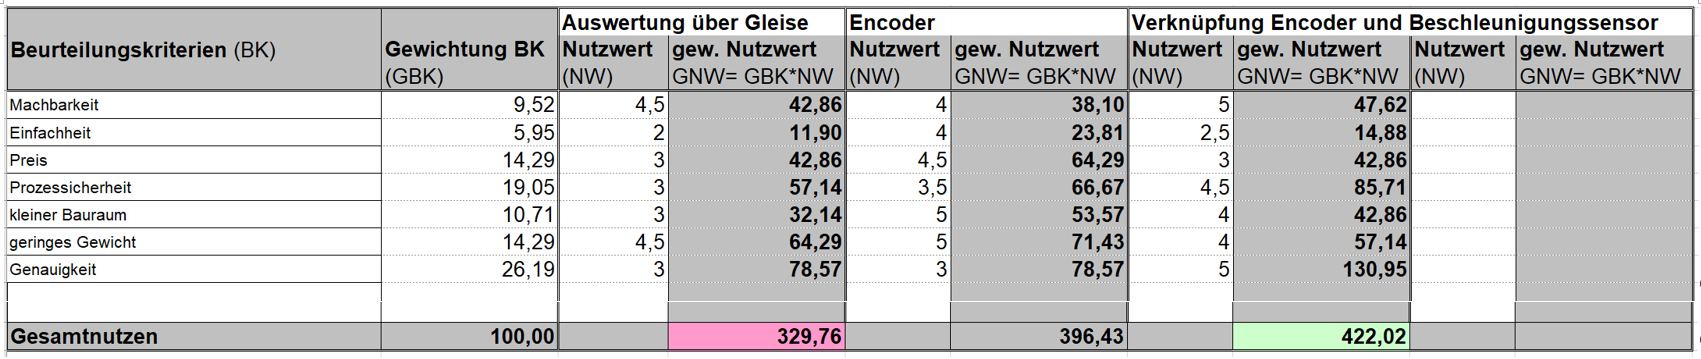
\includegraphics[width=1.0\textwidth]{Nutzweranalyse_Fahrdaten_Geschwindigkeit.png}
        \caption {Nutzwertanalyse Fahrdaten Geschwindigkeit}
        \label{fig:fahr_nutzwertanalyse_geschwindigkeit}
    \end{figure}

    \subsection{Fahrdaten: Positionen}
    Das Auswerten der Position erlaubt eine virtuelle Abbildung der Fahrbahn und somit eine optimierte zweite Runde durch Vorhersage von Kurven und Geraden.


    \textbf{Übersicht Konzepte}\\
    Es werden der verschiedene Ansätze mit verschiedenen Sensoren betrachtet. Zu jeder Möglichkeit werden Vor- und Nachteile aufgelistet und Risiken analysiert.
    \begin{itemize}
        \item Verknüpfung mit Beschleunigungssensor
        \item GPS
        \item Verknüpfung Encoder und Beschleunigungssensor
    \end{itemize}

    \subsubsection{Verknüpfung mit Beschleunigungssensor}
    Über den Beschleunigungssensor kann man die aktuelle Position auf der Fahrbahn berechnen. Die zurückgelegte Strecke errechnet sich durch Integration der Geschwindigkeit oder durch zweifache Integration der Beschleunigung.\\
    Unter der Annahme, dass zu beginn der Messung zum Zeitpunkt $t = 0$ die zurückgelegte Strecke $0$ ist $(s_0 = 0)$ kann die Geschwindigkeit zum Zeitpunkt $t$ bestimmt werden mit $$s(t) = \int_{0}^{t} v(x) dx$$.\\
    Da aber auf einem Digitalen System die Daten nur zu diskreten Zeitpunkten ausgewertet werden können ergibt sich dann eine Summen der Geschwindigkeiten zum Zeitpunkt $k$ $$s[k] = \sum_{i=0}^{k}v[i] \Delta t$$\\
    Die Geschwindigkeit wird gemäss Kapitel \ref{fahr_geschwindigkeit} bestimmt.

    \begin{flushleft}
        \begin{table}[H]
        \begin{tabular}{ | l | p{11cm} |}
        \hline
        \textbf{Problemstellung} & Fahrdaten: Position \\ \hline
        \textbf{Disziplin} & Elektrotechnik \\ \hline
        \textbf{Lösungskonzept} & Verknüpfung mit Beschleunigungssensor\\ \hline
        \textbf{Komponente} & \begin{itemize}
            \item Sensor zum erfassen der Geschwindigkeit
            \item Berechnung auf dem Controller
            \end{itemize}\\ \hline
        \textbf{Bewertung} &  \begin{itemize}
                                \item[+] keine weiteren Sensoren nötig
                                \item[-] Messfehler werden über die Zeit addiert
                              \end{itemize} \\ \hline
        \end{tabular}
        \caption{Konzeptbeurteilung: Position Verknüpfung mit Beschleunigungssensor}
        \label{tab:fahr_pos_Beschleunigung}
    \end{table}
    \end{flushleft}

    \subsubsection{GPS}
    Beim GPS wird die Position über das Anpeilen mehrerer Satelliten geschätzt.
    Dies hat zum Nachteil, dass die erhaltenen Daten eine Abweichung von mehreren Zentimetern aufweisen können.
    Das dazu benötigte Modul würde zusätzlich kosten und Platz einnehmen.

    Mathematisch würde anhand der erhaltenen X- und Y-Koordinaten die Verschiebung auf der Fahrbahn berechnet werden.
    In einem von uns vorgegebene Intervall werden Koordinaten ausgelesen und zu einer Abbildung der Fahrbahn gestaltet.

    \begin{flushleft}
        \begin{table}[H]
        \begin{tabular}{ | l | p{11cm} |}
        \hline
        \textbf{Problemstellung} & Fahrdaten: Position \\ \hline
        \textbf{Disziplin} & Elektrotechnik \\ \hline
        \textbf{Lösungskonzept} & GPS\\ \hline
        \textbf{Komponente} & \begin{itemize}
            \item GPS Modul
            \end{itemize}\\ \hline
        \textbf{Bewertung} &  \begin{itemize}
                                \item[+] Relativ Einfach
                                \item[+] Effizient
                                \item[-] Teuer
                                \item[-] Eher ungenau
                                \item[-] schlechter Empfang im Gebäude 
                              \end{itemize} \\ \hline
        \end{tabular}
        \caption{Konzeptbeurteilung: Position GPS}
        \label{tab:fahr_pos_gps}
    \end{table}
    \end{flushleft}

    \subsubsection{Lichtraumprofil mit Rundenerkennung}
    Bei jedem Durchfahren eines Lichtraumprofils wird bestimmt in welchem Teilbereich der Fahrbahn sich der Wagen befindet.
    Dies ist eine sehr ungenaue Angabe der Position und auch nicht weiter hilfreich, als die Anzahl Runden zu zählen.
    Es kann gut mit anderen Konzepten verknüpft werden um das Ende einer Runde zu bestimmen.

    Mithilfe einer Kamera oder eines Distanz-Sensors kann ein Lichtraumprofil erkannt werden.


    \begin{flushleft}
        \begin{table}[H]
        \begin{tabular}{ | l | p{11cm} |}
        \hline
        \textbf{Problemstellung} & Fahrdaten: Position \\ \hline
        \textbf{Disziplin} & Elektrotechnik \\ \hline
        \textbf{Lösungskonzept} & Lichtraumprofil mit Rundenerkennung\\ \hline
        \textbf{Komponente} & \begin{itemize}
            \item Sensorik zur Lichtraumprofilerkennung
            \end{itemize}\\ \hline
        \textbf{Bewertung} &  \begin{itemize}
                                \item[+] Einfach
                                \item[+] Zuverlässig
                                \item[+] Kann kombiniert werden
                                \item[-] Sehr ungenau
                              \end{itemize} \\ \hline
        \end{tabular}
        \caption{Konzeptbeurteilung: Lichtraumprofil mit Rundenerkennung}
        \label{tab:fahr_pos_Lichtraumprofilerkennung}
    \end{table}
    \end{flushleft}

    \subsubsection{Entscheid}
    Mithilfe der Nutzwertanalyse in Abbildung \ref{fig:fahr_nutzwertanalyse_positiont} konnte ein Entscheid getroffen werden.\\
    Die Entscheidung für die Positionsauswertung über den Beschleunigungssensor als 1. Variante und Lichtraumprofil mit Rundenerkennung als 2. Variante entschieden. Dies ist unter anderem durch Kosten und Platzgründe zustande gekommen. 
        
    \begin{figure}[H]
        \centering
        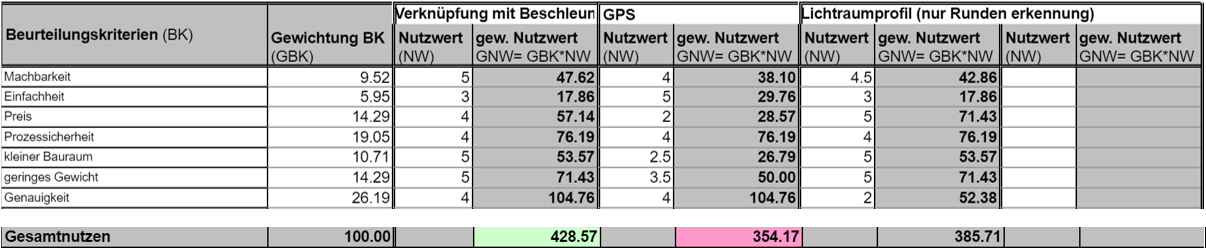
\includegraphics[width=1.0\textwidth]{Nutzweranalyse_Fahrdaten_Position.png}
        \caption {Nutzwertanalyse Fahrdaten Position}
        \label{fig:fahr_nutzwertanalyse_positiont}
    \end{figure}


    \end{document}